\documentclass[%
reprint,nofootinbib,
amsmath,amssymb,
aps,
]{revtex4-1}
\usepackage{graphicx}% Include figure files
\usepackage{dcolumn}% Align table columns on decimal point
\usepackage{bm}% bold math
\usepackage[utf8]{inputenc}
\usepackage{listings}
\usepackage{amsmath}
\usepackage{physics}
\usepackage{booktabs}
\usepackage{float}
\usepackage[bottom]{footmisc}
\usepackage{scrextend}
\bgroup
\def\arraystretch{1.3}
\newcommand{\HRule}{\rule{\textwidth}{0.5mm}}
\makeatletter
\newcommand*{\rom}[1]{\expandafter\@slowromancap\romannumeral #1@}
\makeatother

\begin{document}
\onecolumngrid

\begin{center}
	\large\textbf{The Ising Model\\ \small{Studies of phase transitions in magnetic systems}}
\end{center}
\vspace{5mm}

\begin{center}
	\small{$^1$ Oline A. Ranum}\\
\end{center}

\begin{center}
	\small{$^1$ University of Oslo, Institute of physics, 
		olinear@student.matnat.uio.no}
\end{center}

\begin{center}
	\textit{\today}
\end{center}
\vspace{7mm}
\noindent 
\HRule \vspace{2mm}\\
The main objective of this paper is to 
\vspace{1.5mm}  \\
\HRule
\vspace{0.3cm}

\twocolumngrid 
\section{Introduction}
The Icing model was first developed
The Icing model describes
I first present theory 

The Icing model has been extremely popular, with applications spanning from studies of phase transitions to simulations in statistics. 
 \newpage. \newpage 
\section{Theory} \noindent 
\subsection{The Ising model} \noindent 
The Ising model is a ferromagnetic model consisting of discrete variables that represent magnetic dipole moments of atomic spin, tha is suitable for studies of phase transitions at finite temperatures. For a given critical temperature, the Ising model exhibits a phase transition from a magnetic phase to a phase with zero magnetization. The model is therefor a binary system where the objects at each lattice site can only take two values, for instance -1 and 1. In one or two dimensions the Ising model has analytical solutions to several expectation values and it gives a qualitatively good understanding of several types of phase transitions. \\ \indent 
In its simplest form the Ising model describes the energy of a specified system configuration as  
\begin{equation}\label{isemodel}
	E = -J\sum_{\expval{kl}}^{N}s_ks_l -\Lambda \sum_{k}^{N} s_k
\end{equation}
where $s_k = \pm 1$, N is the total number of spin and $J$ is a coupling constant expressing the strength of the interaction between neighboring spins. The formulation $\expval{kl}$ indicates that we sum over nearest neighbors only. The parameter $\Lambda$ is an external magnetic field interacting with the magnetic moment set up by the spins. The last contribution is omitted when there is no externally applied field.\\ \indent 
For a ferromagnetic ordering $J> 0$, meaning it is energetically favorable for neighboring spins to be aligned. It is a feature that for significantly low temperatures leeads to a cooperative phenomenon called spontaneous magnetization. In other words, through interactions between nearest neighbors, a given magnetic moment can influence tha alignment of spins that are separated from the given spin by a macroscopic distance. The magnetisation in such a system can be modeled as the sum over all spins for a given configuration $i$
\begin{equation}\label{mf}
M_i = \sum_{j = 1}^{N}s_j
\end{equation}

\subsection{Periodic boundary conditions} \noindent 
For small systems, the way that the boundaries of the system are treated has an effect on the calculations. Periodic boundary conditions implies that the neighbor to the right of value $s_N$ is assumed to take the value of $s_1$, or equivalently that the neighbor to the left of $s_1$ takes the value $s_N$. 


\subsection{Thermodynamical systems} \noindent 
Finite, quantized systems with discrete properties will in general have a finite set of possible configurations $i$. Systems where the temperature for such a system is held constant, it is describable by the standard relations of Boltzmann statistics. I. e. the ensemble of micro state at any given temperature has the probability distribution \vspace{1mm}
\begin{equation}
P_i(\beta) = \dfrac{e^{-\beta E_i}}{Z}
\end{equation}  \vspace{1mm}
where $\beta^{-1} = kT$ with $k$ being the Boltzmann constant, T the temperature of the system and $E_i$ the energy of the microstate $i$. It follows that the partition function for the canonical ensemble is defined by\vspace{1mm}
\begin{equation}\label{pf}
	Z = \sum_{i = 1}^{M}e^{-\beta E_i}
\end{equation}\vspace{1mm}
where M is the number of micro-states $i$. In general, such a system will have properties $X$ who's moments follow \vspace{1mm}
\begin{equation}
	\expval{X} = \dfrac{1}{Z}\sum_iX_ie^{-\beta E_i}
\end{equation}\vspace{1mm}
In case of the expectation value of the energy, the following formula is also useful\vspace{1mm}
\begin{equation}\label{ev}
 \expval{E} = -\dfrac{\partial\ln Z}{\partial\beta}
\end{equation}\vspace{1mm}
The specific heat capacity $C_V$ of a system would be \vspace{1mm}
\begin{equation}\label{cv}
C_V = \dfrac{\beta}{T}\qty[\expval{E^2}-\expval{E}^2]
\end{equation}\vspace{1mm}
and the susceptibility \vspace{1mm}
\begin{equation}\label{chi}
\chi = \dfrac{\beta}{T}\qty(\expval{M^2}- \expval{M}^2) \vspace{1mm}
\end{equation} 
\hspace{6.cm}[M. Jensen, 2015]


\subsection{Ising model on 2x2 grid} \noindent 
For small systems, the boundary conditions matter. In the following it is assumed that the system is on a $2\times2$ lattice, with periodic boundary conditions. The arrangement of such a system is illustrated in figure \ref{si}, where each individual spin $s_i$ can either be up or down. \\ 
\begin{figure}
	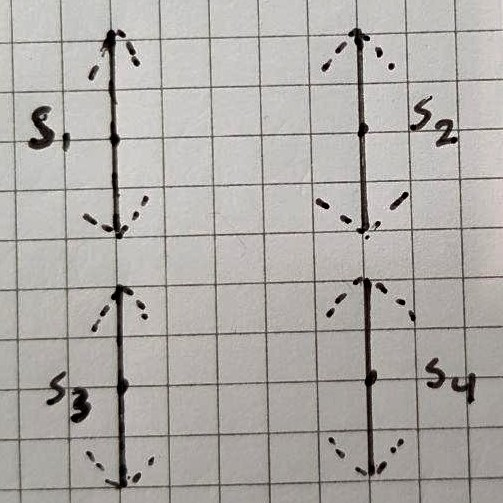
\includegraphics[width = \columnwidth]{si.jpg}
	\caption{Illustration of the possible spin-configurations of the $2\times 2$ Ising model. Each individual spin $i$ can either be up or down.\label{si}}
\end{figure}
For a $2\times 2$ grid there exist $2^4 = 16$ different configurations. Various relevant properties of the $2\times 2$ system are presented below. Here, the quantities are simply presented, whereas their full derivation can be found in the appendix. The analytical partition function for this system 
\begin{equation} \vspace{1mm}
	Z =  4\cosh(8J\beta) + 12 
\end{equation} \vspace{1mm}
The energy expectation values are \vspace{1mm}
\begin{align}
	\expval{E} = -\dfrac{32J}{z}\sinh(8J\beta)
\end{align}\vspace{1mm}
\begin{align}
	\expval{E^2} = \dfrac{258J^2}{Z}\cosh(8J\beta)
\end{align}\vspace{1mm}
It follows from equation \ref{cv} that \vspace{1mm}
\begin{align}
	C_V= \dfrac{\beta}{T}64J^2\qty[\dfrac{\cosh(8J\beta)}{\cosh(8J\beta) + 3}  -\qty(\dfrac{\sinh(8J\beta)}{\cosh(8J\beta) + 3 })^2]\nonumber  \\&\nonumber \\
\end{align}\vspace{1mm}
The magnetization expectation values becomes \vspace{1mm}
\begin{align*}
	\expval{M} =  0
\end{align*}\vspace{1mm}
\begin{align*}
\expval{\abs{M}} =  \dfrac{2e^{8J\beta}}{\cosh(8J\beta) + 3 }
\end{align*}\vspace{1mm}
\begin{align*}
\expval{M^2} = \dfrac{8e^{8J\beta} + 8}{\cosh(8J\beta) + 3}
\end{align*}\vspace{1mm}
Then, according to equation \ref{chi} the susceptibility is \vspace{1mm}
\begin{align}
	\chi = \dfrac{\beta}{T}\dfrac{8e^{8J\beta} + 8}{\cosh(8J\beta) + 3}
\end{align}
\subsection{The metropolis algorithm}

\section{Method} \noindent 
Initially, it is assumed that there is only two spins in each dimension and that the boundaries are subjected to periodic conditions. Equation \ref{ef} is used to calculate the energy expectation value for all possible configurations and equation \ref{mf} is used to estimate the mean magnetization $\abs{M}$. The specific heat $C_V$ and susceptibility $\chi$ is estimated as functions of T with respectively equation \ref{cv} and \ref{sf}. The results of the calculation are used as benchmark calculations in the next step. 
The results presented in table \ref{bc} is the analytical evaluation of selected parameters of a $2\times2$ lattice.
\newpage 
\section{Results} \noindent
The results of estimating a $2\times 2$ Ising model Monte Carlo simulation with the Metropolis algorithm is presented in table \ref{2b}. It is evident that approximately $N=10^7$ was sufficient to make a good approximation to the analytical values. 
\begin{table}[!h]
	\caption{\label{2b}Results per spinz of a Metropolis Algorithm using the Ising model on a $2\times 2$ system with 16 various configurations as a function of N. The analytical expectation values are given at the bottom of the table as E. }
	\begin{tabular}{|c|c|c|c|c|c|c|c|} \hline 
		\textbf{N}  & \hspace{1mm}	$\expval{\mathbf{E}}$ \hspace{1mm} & \hspace{1mm}$\expval{\mathbf{E^2}}$ \hspace{1mm} & \hspace{1mm}	$\expval{\mathbf{M}}$\hspace{1mm}  &	\hspace{1mm} $\expval{\mathbf{M^2}}$ \hspace{1mm}  &	\hspace{1mm}$\expval{\abs{\mathbf{M}}} $\hspace{1mm} & \hspace{2mm}$\mathbf{\chi}$	\hspace{2mm} & \hspace{2mm}	\textbf{C}$_V$\hspace{2mm} \\ \hline 
		&&&&&&&\\
		10$^4$   &          -1.9952   & 15.9617  &  0.8206 &   15.9680 &   3.9936&   0.0381 &   1.6071\\
		10$^5$   &          -1.9963   & 15.9701  &  -0.5715 &   15.9751 &   3.9950&   0.0298 &   3.5324\\  
		10$^6$   &          -1.9959   & 15.9674  &  -0.1322 &   15.9729 &   3.9946&   0.0325 &   3.9499\\  
		10$^7$   &          -1.9960   & 15.9680  &  0.0064 &   15.9733 &   3.9947&   0.0320 &   3.9908\\ 
		10$^8$   &          -1.9960   & 15.9678  &  0.0201 &   15.9732 &   3.9946&   0.0321 &   3.9928\\
		&&&&&&&\\ \hline 
		E &-1.996 & 16.0926  &0.&     15.9732&  3.992 &  0.0321 & 3.9933 \\ \hline 
	\end{tabular}
\end{table}\\ 

\onecolumngrid
\begin{figure*} 
	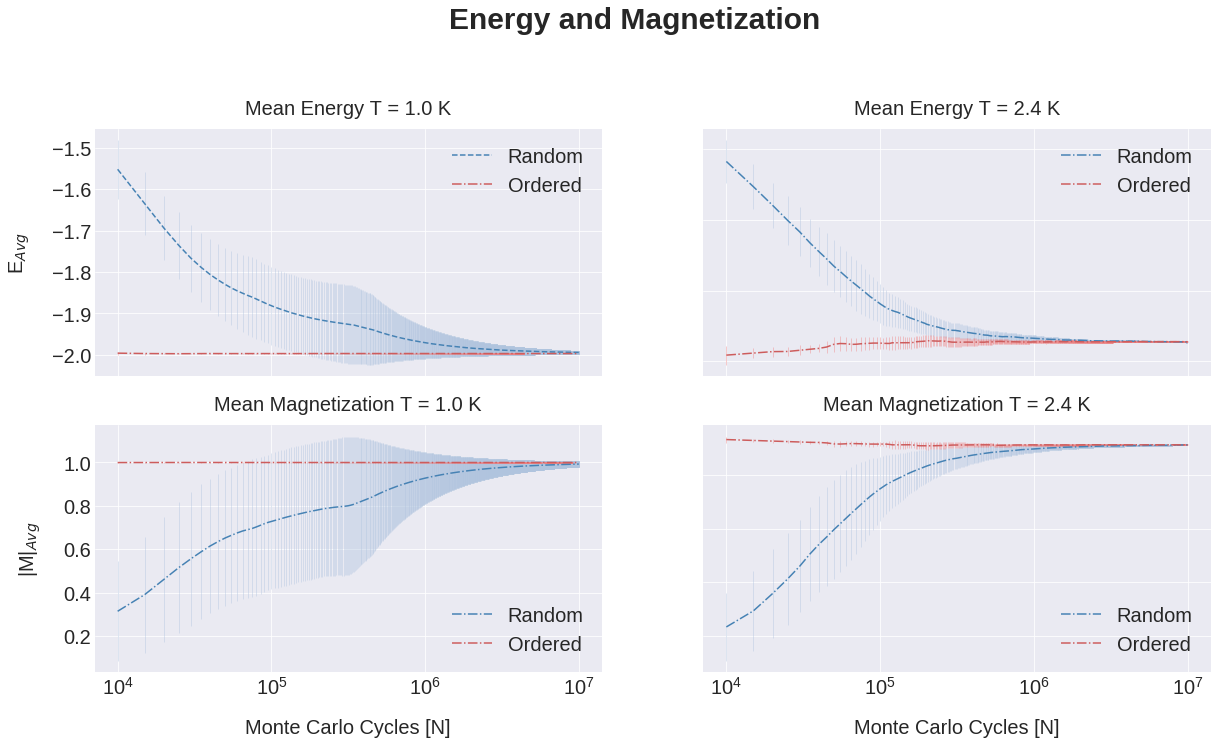
\includegraphics[width = \textwidth]{Figures/4C1.png} 
	\caption{\centering \label{4C1}Average energy and magnetization per spin as function of Monte Carlo cycles. The errorbar represents the standard deviation of 10 independent test runs.}
\end{figure*}
\twocolumngrid

The equilibration time $t_{eq}$, or the number of Monte Carlo cycles needed to reach this equilibrium position, is roughly $10^7$ cycles.  


\begin{figure*} 
	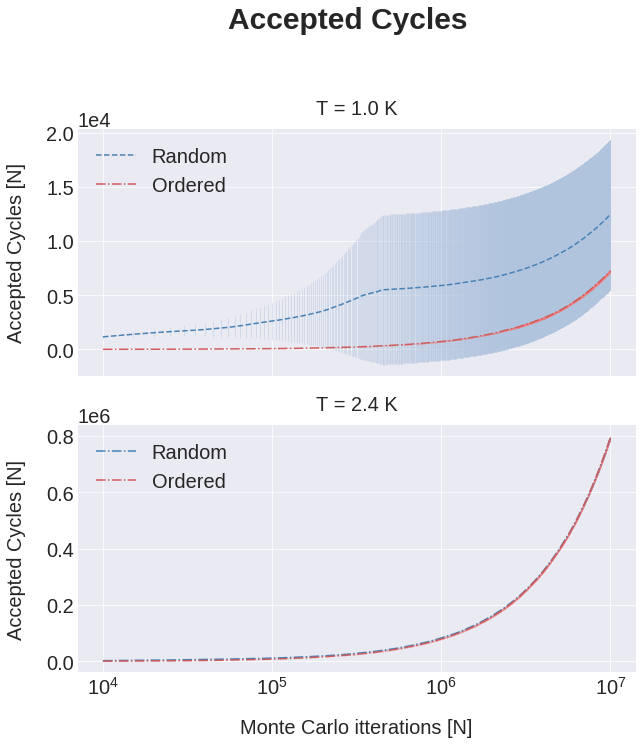
\includegraphics[width = \textwidth]{Figures/Plot2.png} 
	\caption{\centering \label{4C1}Average energy and magnetization per spin as function of Monte Carlo cycles. The errorbar represents the standard deviation of 10 independent test runs.}
\end{figure*}

\begin{figure*} 
	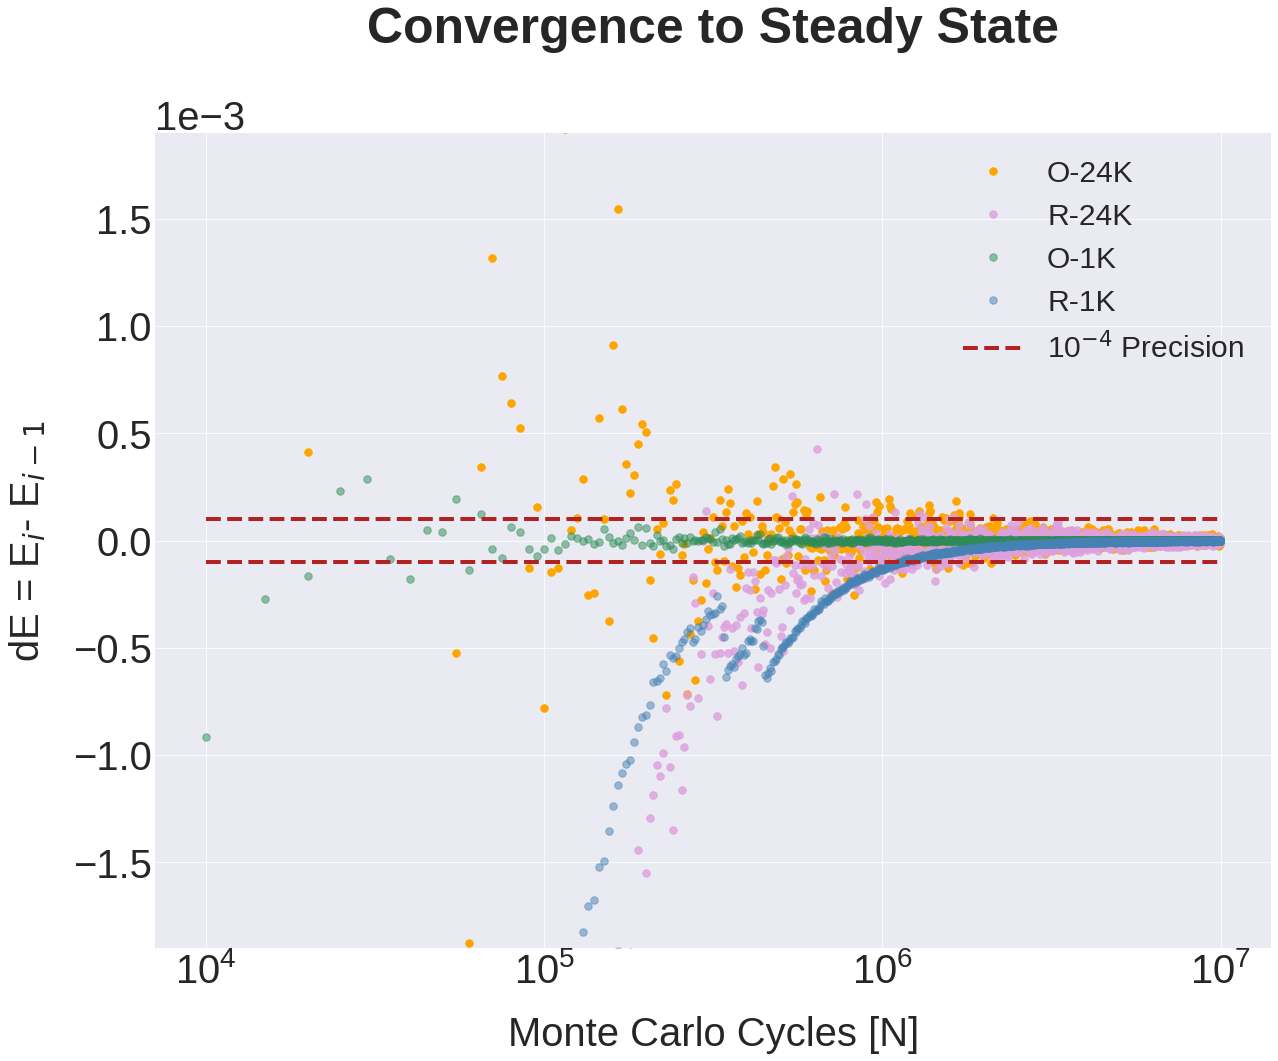
\includegraphics[width = \textwidth]{Figures/Plot3.png} 
	\caption{\centering \label{4C1}Average energy and magnetization per spin as function of Monte Carlo cycles. The errorbar represents the standard deviation of 10 independent test runs.}
\end{figure*}
\newpage.
\newpage.
\newpage.
\section{Discussion} \noindent 
\section{Conclusion} \noindent 
\newpage . \newpage
\onecolumngrid 
\section{References} \noindent
\newpage
\section{Appendix} \noindent
\subsection{Derivation of thermo-physical quantities for a $2\times 2$ lattice grid}
Each energy state for the various configurations are determined by equation \ref{isemodel}, who for the specific $2\times2$ lattice grid is
\begin{align*}
E_i  =& -J[s_1s_2 + s_1s_3 + s_2s_1+s_2s_4+s_4s_2+s_4s_3 + s_3s_1 + s_3s_4] \nonumber \\
= &-2J[s_1s_2 + s_2s_3 + s_3s_4 + s_4s_1]
\end{align*}\vspace{1mm} 
One can use this relation to estimate the analytical partition function \footnote{By identity: $2\cosh(\alpha) = e^{-\alpha} + e^{\alpha}$}
\begin{align*}
Z = \sum_{i = 1}^{16}e^{2J\beta[s_1s_2 + s_2s_3 + s_3s_4 + s_4s_1]}
=&  2e^{-8J\beta} + 2e^{8J\beta} + 12e^0\nonumber \\
= & 4\cosh(8J\beta) + 12 
\end{align*} 
Using equation \ref{ev} it is evident that the energy expectation value for the system becomes 
\begin{align*}
\expval{E} = -\dfrac{\partial ln Z}{\partial \beta} = -2\dfrac{\partial}{\partial \beta}\ln{[e^{-8J\beta} + e^{8J\beta}]} =& -\dfrac{16J}{Z}[e^{8J\beta} - e^{-8J\beta}] \\ 
& = -\dfrac{32J}{z}\sinh(8J\beta)
\end{align*}
Table \ref{bc} shows all configurations and their corresponding energy $E_i$ and magnetization $M_i$

\begin{table}[!h]
	\caption{\label{bc} The 16 configurations for a $2\times 2$ Ising model on a 2D lattice. The energy $E_i$ and magnetization $M_i$ for each configuration $i$ is provided.}
	\begin{tabular}{|c|c|c|c|} \hline 
		S$_i$&S$_\uparrow$ & \textbf{$E_i$} [J]&$ M_i$ [\#] \\ \hline   
		0& $\uparrow\uparrow\uparrow\uparrow$ &-8J&4\\
		1&$\uparrow\uparrow\uparrow\downarrow$ & 0&2\\
		2&$\uparrow\uparrow\downarrow\uparrow$ &0&2\\
		3&$\uparrow\downarrow\uparrow\uparrow$ &0&2\\
		4&$\downarrow\uparrow\uparrow\uparrow$ &0&2\\
		5&$\uparrow\uparrow\downarrow\downarrow$ &0&0\\
		6&$\downarrow\downarrow\uparrow\uparrow$ &0&0\\
		7&$\uparrow\downarrow\uparrow\downarrow$ &0&0\\
		8&$\downarrow\uparrow\downarrow\uparrow$ &0&0\\
		9&$\downarrow\uparrow\uparrow\downarrow$ &8J&0\\
		10&$\uparrow\downarrow\downarrow\uparrow$ &8J&0\\
		11&$\uparrow\downarrow\downarrow\downarrow$ &0&-2\\
		12&$\downarrow\uparrow\downarrow\downarrow$ &0&-2\\
		13&$\downarrow\downarrow\uparrow\downarrow$ &0&-2\\
		14&$\downarrow\downarrow\downarrow\uparrow$ &0&-2\\
		15&$\downarrow\downarrow\downarrow\downarrow$ &-8J&-4\\\hline 
	\end{tabular}
\end{table}


The specific heat capacity of this system can be calculated using equation $cv$, 
\begin{align}
\expval{E^2} = \dfrac{1}{Z}\sum_{i=1}^{16}E_ie^{-\beta E_i}  = & \dfrac{128J^2}{Z}(e^{8J\beta} + e^{-8J\beta}) \\
=& \dfrac{258J^2}{Z}\cosh(8J\beta)
\end{align}
It follows that 
\begin{align}
C_V =& \dfrac{\beta}{T}\qty[\dfrac{258J^2\cosh(8J\beta)}{4\cosh(8J\beta) + 12 }  -\qty(-\dfrac{32J\sinh(8J\beta)}{4\cosh(8J\beta) + 12 })^2] \nonumber \\
= & \dfrac{\beta}{T}64J^2\qty[\dfrac{\cosh(8J\beta)}{\cosh(8J\beta) + 3}  -\qty(\dfrac{\sinh(8J\beta)}{\cosh(8J\beta) + 3 })^2]\nonumber \\ \nonumber & \\ & 
\end{align}
The mean magnetization becomes 
\begin{align*}
\expval{M} =& \dfrac{1}{Z}\sum_{i = 1}^{16} M_ie^{-\beta E_i} \\ 
= & \dfrac{1}{Z}\qty(4e^{8J\beta} +4\times 2e^0 + 4\times(-2)e^0 -4e^{8J\beta}) \\
= & 0
\end{align*}
\begin{align*}
\expval{\abs{M}} =& \dfrac{1}{Z}\sum_{i = 1}^{16} \abs{M_i}e^{-\beta E_i} \\ 
= & \dfrac{1}{Z}\qty(4e^{8J\beta} +4\times 2e^0 + 4\times2e^0 +4e^{8J\beta}) \\
= & \dfrac{8e^{8J\beta}}{4\cosh(8J\beta) + 12 } \\
= & \dfrac{2e^{8J\beta}}{\cosh(8J\beta) + 3 }
\end{align*}
\begin{align*}
\expval{M^2} =& \dfrac{1}{Z}\sum_{i = 1}^{16} M_i^2e^{-\beta E_i} \\ 
= & \dfrac{1}{Z}\qty(16e^{8J\beta} +4\times 4e^0 + 4\times4e^0 + 16e^{8J\beta}) \\
= & \dfrac{8e^{8J\beta} + 8}{\cosh(8J\beta) + 3}
\end{align*}
Yielding the susceptibility 
\begin{align}
\chi =& \dfrac{\beta}{T}\qty(\expval{M^2}- \expval{M}^2)\\
=& \dfrac{\beta}{T}\dfrac{8e^{8J\beta} + 8}{\cosh(8J\beta) + 3}
\end{align}

 
\end{document}